\section{Large-Scale Simulation Results}
\label{sec:eval}

To evaluate our techniques in a large scale area (a few kms square),
we conducted simulations over a geographic area using path-loss values
from the Longley-Rice propagation model generated by
open sourse software SPLAT!~\cite{splat}. We describe the simulation setting below and
discuss the results.

\subsection{Settings}

\para{Generating Probability Distributions.} To evaluate our
techniques over a large area with 100s of sensor nodes, we need to run
simulations with an assumed propagation model. We use the well-known
Longley-Rice ~\cite{chamberlin82} Irregular Terrain With Obstruction Model (ITWOM), 
which is a complex model of wireless
propagation based on many parameters including locations, terrain
data, obstructions and soil condition etc. and such.
%%%%%%%%%%%%
We consider an area of 4km $\times$ 4km in the NY state and use the
800 MHz band for SPLAT! We discretize the area using 40 vertical and
40 horizontal grid lines---yielding 1600 cells each of size 100m
$\times$ 100m.
%\red{Each cell represents a discrete location.}
%%%%%%
To generate a probability distribution (PD) at a sensor location $x$
due to a transmitter at location $l$ transmitting at power $\pstar$,
we compute the received power at $x$ using transmit power minus path-loss from SPLAT!, and use it as the mean of the probability distribution. For the
complete PD, we assume Gaussian distributions and use a standard
deviation between 1 and 3, with higher values for pairs $(x,l)$ with
smaller distance.
%%%%%%
As mentioned before, the PD due to multiple simultaneous transmitters
can be computed as just a ``sum'' of the Gaussian distributions due to
individual transmitters~\cite{rappaport-2001,mobicom17-splot}.
%% \ble{The expectation of power of the sum of multiple signals is equal
%%  to the sum of power of the individual signals
%%  ~\cite{rappaport-2001}.  ~\cite{mobicom17-splot} validates this by
%%  conducting experiments in the Orbit testbed.}

\para{Algorithms Compared.}  For the \mtl problem, we compare our
\ouralgo algorithm with \splot~\cite{mobicom17-splot} and
\cl~\cite{clustering} (see \S\ref{sec:ipsn-related}). As mentioned
before,~\cite{Quasi-EM} has been shown to be inferior in performance
to both \splot and \cl in their respective works, and thus, not
evaluated here.
%%%%%%
\cl uses $k$-means~\cite{scikit-learn} for clustering, and needs to be
provided with the number of clusters. To do a somewhat fair
comparison, we provide \cl with a {\em range} of the number of
intruders and use the elbow-point method to pick the best
number of clusters/intruders. In particular, the range of intruders
passed to \cl is 1 to $2x$, where $x$ is the actual number of
intruders present.
%%%%%%%%%
\begin{table}[ht]
	\caption{Simulation Evaluation Parameters.}
	\centering
	\begin{tabular}{c c c c}
		\hline\hline
		Param. & Value & Description \\ [0.5ex]
		\hline
		$Q^{'}_{1}$ &  0.6   & Threshold for Procedure 1's hypothesis posterior\\ 
		$Q^{'}_{2}$ &  0.1   & Threshold for Procedure 2's hypothesis posterior\\
		$R$  & 1000 & Transmission radius when power is \pstar, (m) \\
		\pstar & 30  & Transmit power during training, (dBm) \\
		$\delta_p$ & 2  & Range of intruders' power is $[\pstar - \delta_p, \ \pstar + \delta_p]$\\
		\hline
	\end{tabular}
	\label{table:paramaters}
\end{table}

For \splot, we use the same set of parameters values as
in~\cite{mobicom17-splot} except that we use the confined area radius
to be 800m for our large area setting (\cite{mobicom17-splot} only
considered small 15m $\times$ 15m areas; 800m is roughly the maximum
transmission radius in our large-scale setting and other values
yielded worse results).
%%%%%%
Table \ref{table:paramaters} gives the main parameters of \ouralgo
used in our evaluations. Recall that the transmission radius is the
distance between the TX and RX for which the RX's RSS is at the noise
floor (we use -80dBm). \eat{Issues: Threshold for SPLOT, further explain $STD_1$ and
  $STD_2$}

\begin{figure}[ht]
	\centering
	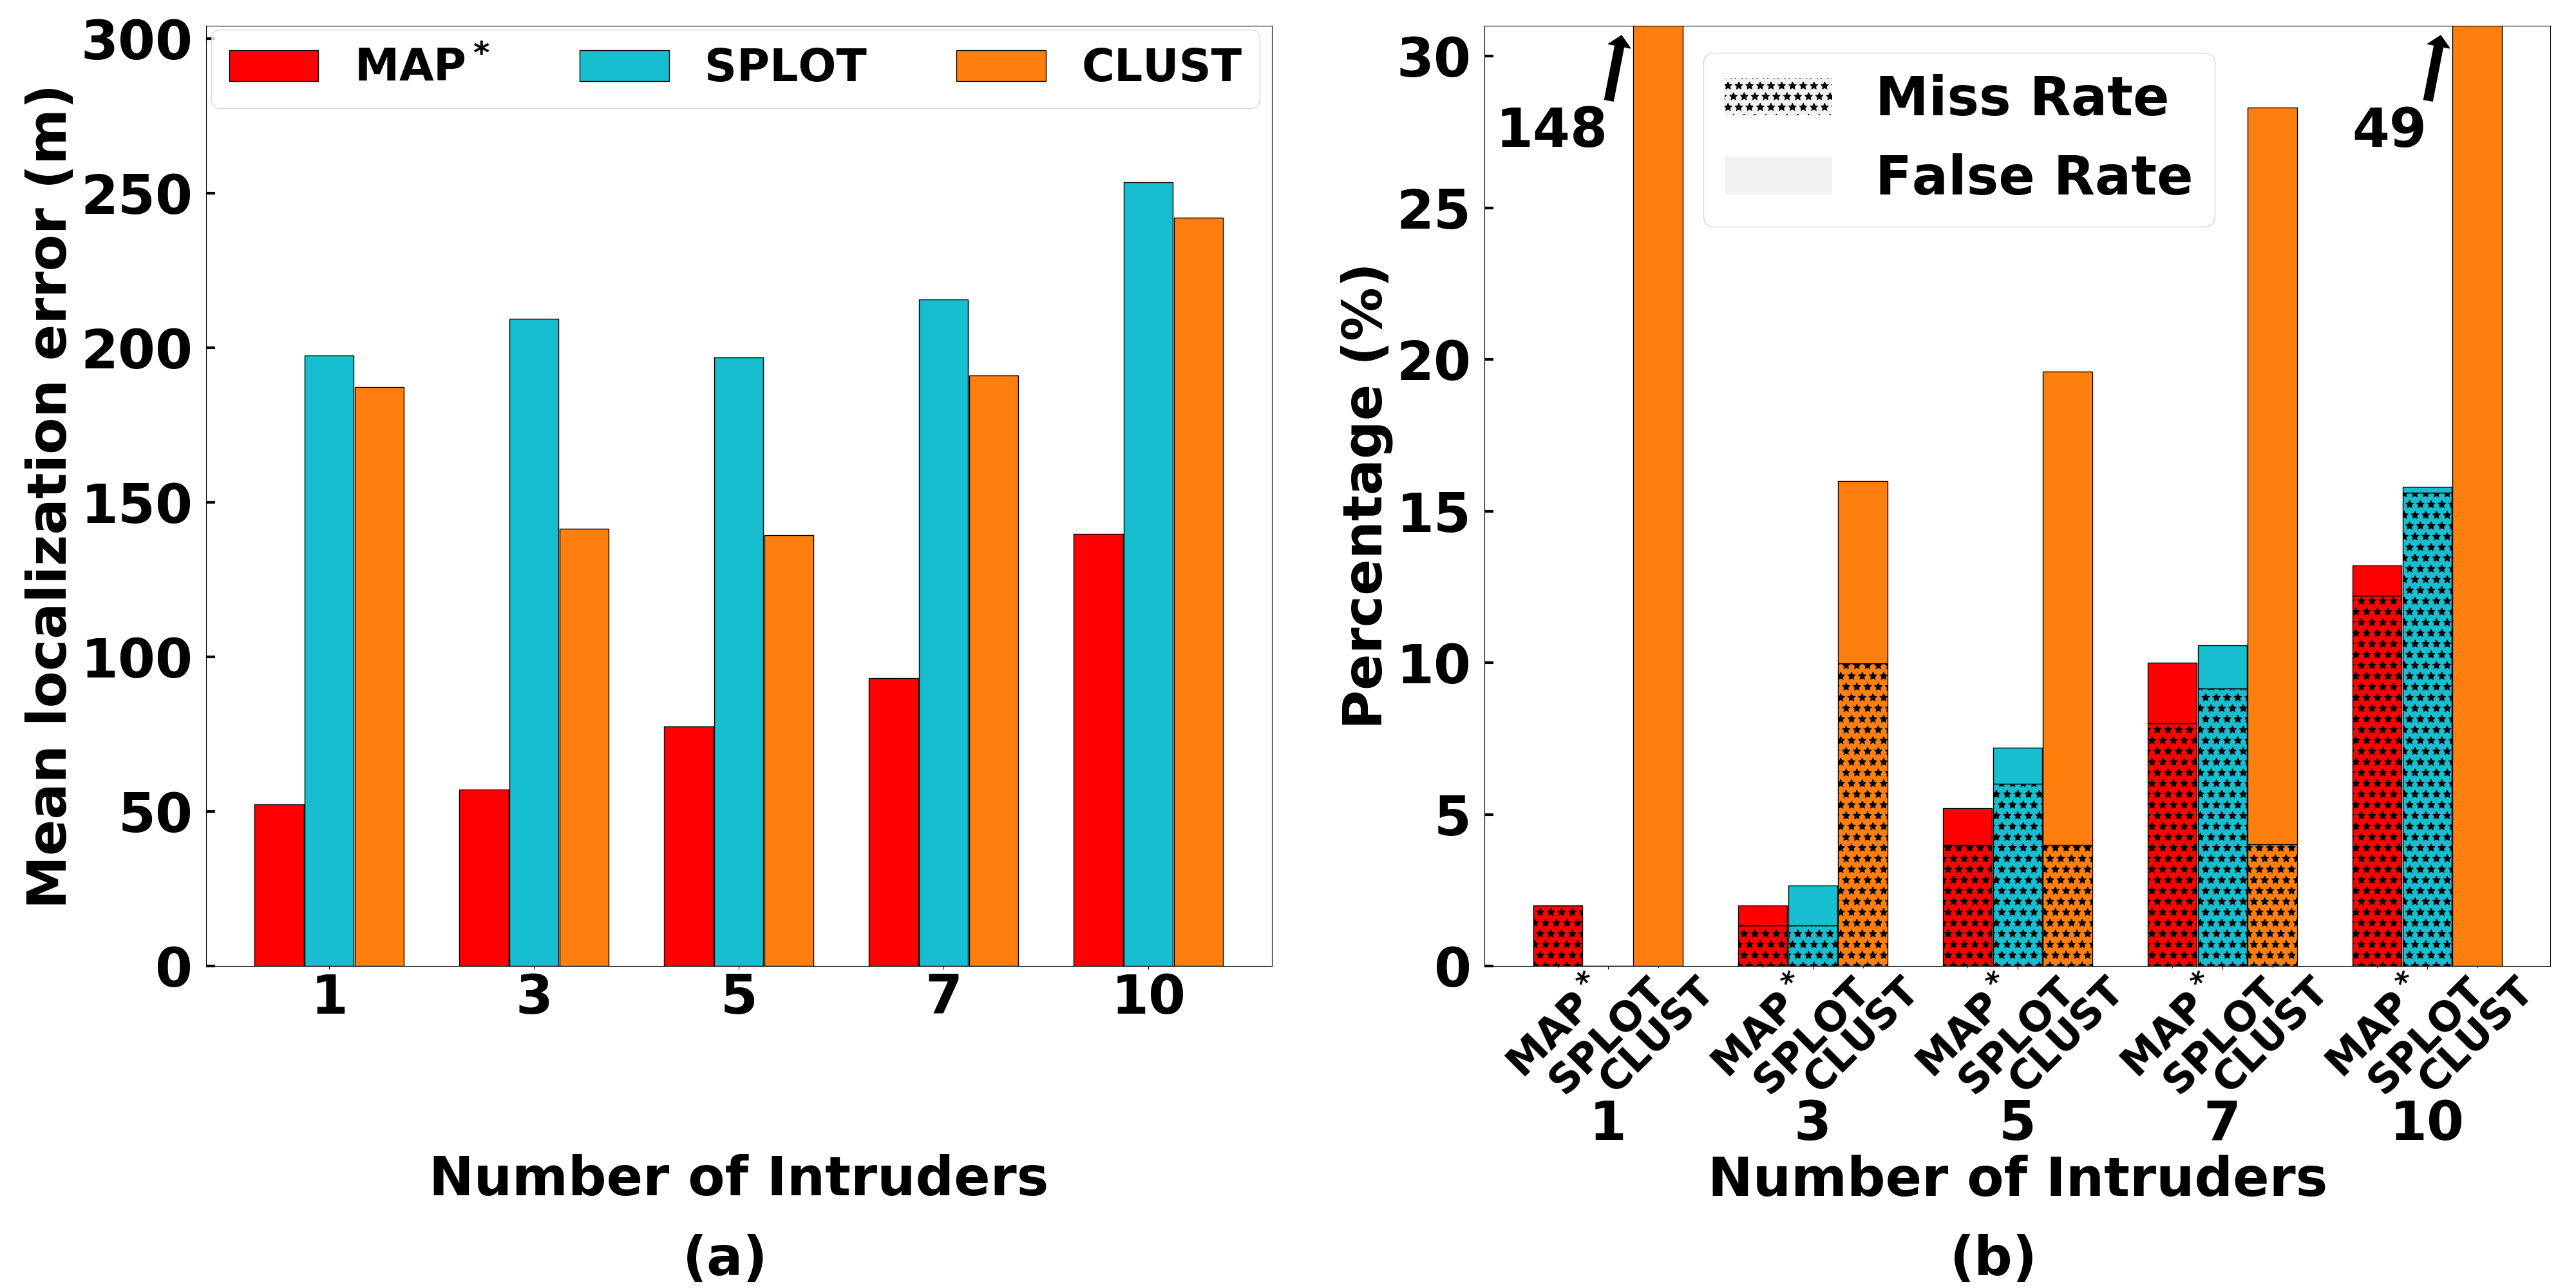
\includegraphics[width=0.8\textwidth]{chapters/ipsn/figures/splat-vary-numintru.png}
	\caption{Localization performance of various algorithms in a large scale area, for varying number of intruders}
	\label{fig:varying-num-intruders}
\end{figure}

\subsection{Five Evaluation Metrics.}
We use the following metrics to evaluate the localization methods. 
\begin{enumerate}
\item Localization error ($\lerr$). 
\item Miss rate ($\mr$).
\item False alarm rate ($\fr$).
\item Power error ($\perr$).
\end{enumerate}
The above metrics are best explained using a simple example. Given a
multi-intruder localization solution, we first compute the $\lerr$ as
the minimum-cost matching in the bi-partite graph over the
ground-truth and the solution's locations, where the cost of each edge
in the graph is the Euclidean distance. We use a simple greedy
algorithm to compute the min-cost matching.
%%%%
The unmatched nodes are regarded as false alarms or misses. E.g., if
there are 4 intruders in reality, but the algorithm predits 6
intruders then it is said to incur 0 misses and 2 false alarms and if
it predicts 3 intruders then it incurs 1 miss and 0 false alarms. The
$\mr$ and $\fr$ metrics are on a per-intruder basis, so in the above
two examples: $\mr$ is 0 and 1/4 and $\fr$ is 2/4 and 0. In the plots, we stack miss rate and false alarm rate together to show the overall difference between the true number of intruders and predicted number of intruders.
%%%%%%%
$\perr$ is the average difference between the predicted power
and the actual power of the matched pair in the above bi-partite
graph. 

Finally for interpolation schemes, we use the metric (5) interpolation error ($\ierr$) defined as the estimated path-loss minus the ground-truth path-loss value.

\subsection{Results}

In this subsection, we evaluate the performance of our techniques for
varying parameter values, viz., number of intruders and sensors in the
field, and training cost.
%%%%%%%%
Here, the training cost is defined relative (specifically, as a
percentage of) to the full training scenario wherein we construct each
of the $1600 \times 1600$ PDs (one for each pair of transmitter and
sensor locations) directly from observations. E.g., $x\%$ training
cost indicates that we construct $1600 \times (16x)$ PDs directly, and
interpolate the remaining $1600 \times (1600-16x)$ PDs; our proposed
interpolation scheme only interpolates for sensor locations.
%%%%%%
In general, when we vary a specific parameter, the other parameters
are set to their default values which are: 9\% for training
cost, 5 for number of intruders, and 240 for number of sensors.
%%%%%
For each experiment, the said number of sensors and intruders are
deployed randomly in the field, with the intruders deployed in the
continuous location domain while the sensors deployed only at the
centers of the grid cells. Each data point in the plots is an
average of 50 experiments.

\begin{figure}[ht]
	\centering
	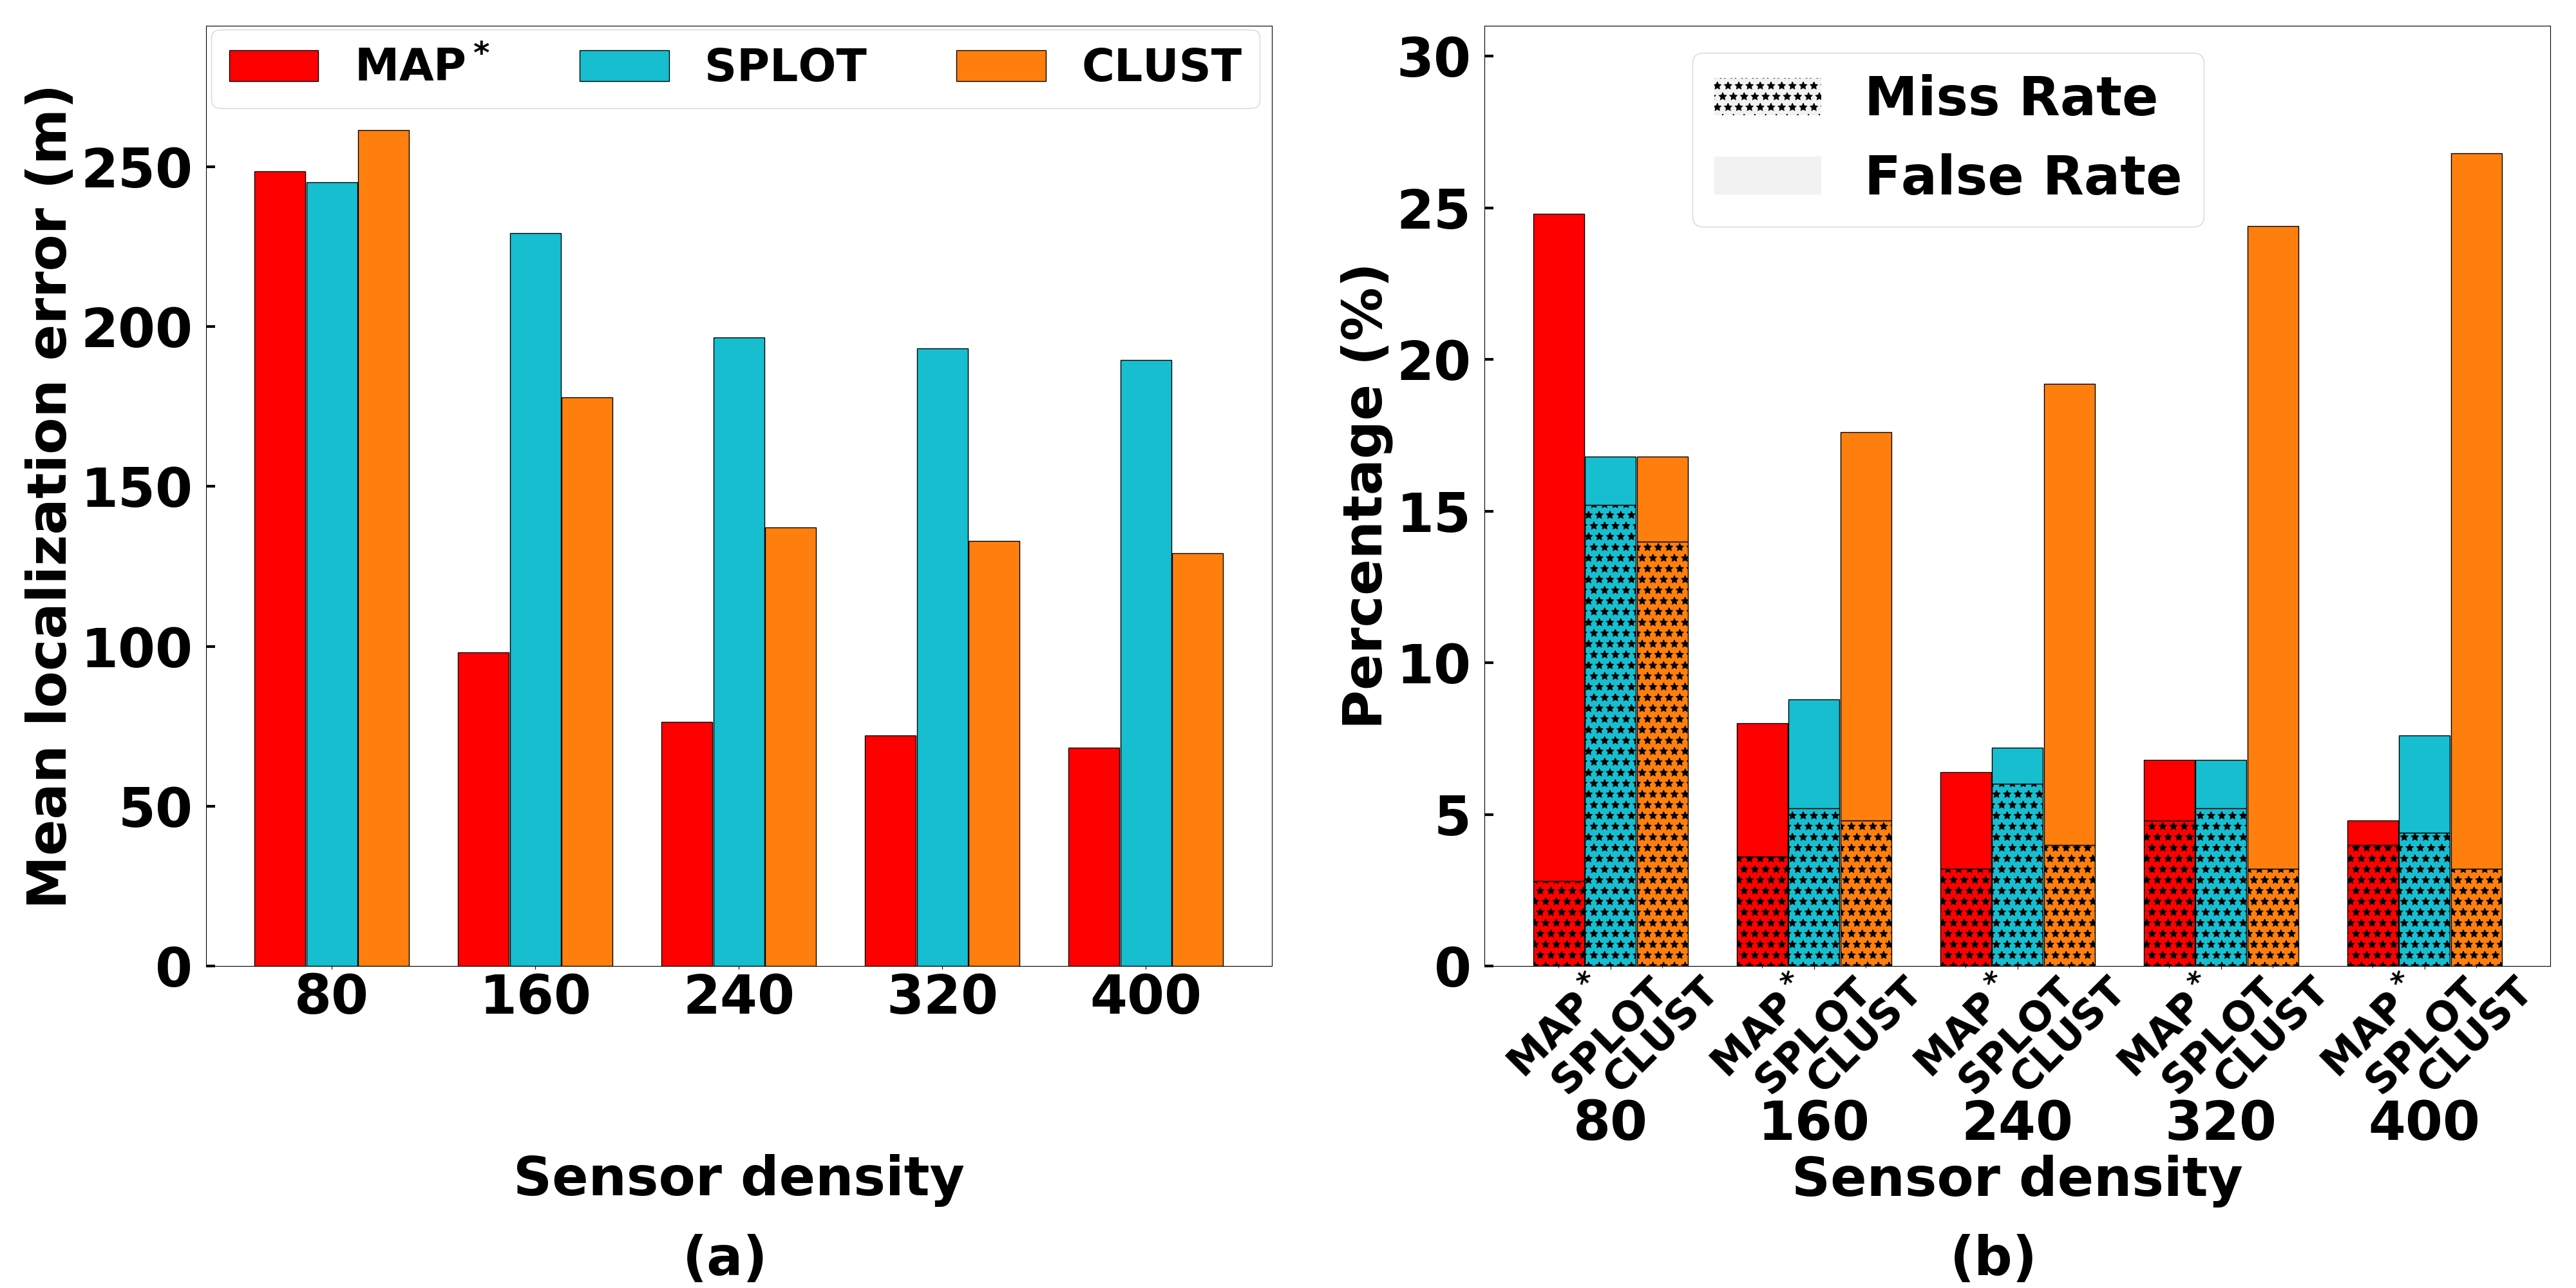
\includegraphics[width=0.8\textwidth]{chapters/ipsn/figures/splat-vary-sendensity.png}
	\caption{Localization performance of various algorithms in a large scale area, for varying sensor density}
	\label{fig:varying-num-sendensity}
\end{figure}

\para{Varying Number of Intruders.}  First, we compare the
localization accuracy of various algorithms for varying number of
intruders.  See Figure \ref{fig:varying-num-intruders}. We vary the
number of intruders from 1 to 10. We observe that the localization
error of \ouralgo is the minimum across the three algorithm. 
The localization error is 45\% -- 74\% less than \splot.
In terms of the $\mr$ and $\fr$, \ouralgo also performs others which confirms the overall performance
of \ouralgo to be the best among the algorithms compared. In terms of
absolute performance, note that the localization error of 50-150m
indicates an error of 1-2 grid cells, and thus is minimal in the
context of the large area of 4km by 4km with 1600 cells and a sensor
population of 240. Investigating further, we observe that misses in
\ouralgo are mostly due to the interpolated PDs (note that only 9\% of
the PDs are constructed from the actual sensor observations, and the
remaining 91\% are interpolated), while \splot's misses are mainly
from the case of two or more intruders being close to each other. This
demonstrates the superior ability of \ouralgo to localize intruders
that are close-by via the designed sequence of Procedures 1 and 2.


\begin{table}
	\caption{\ouralgo Power Error (dB) }
	\centering
	\begin{tabular}{c c c} 
		\hline\hline
		\# Intru. & MAE & ME \\ [0.5ex]
		\hline
		1 & 0.56  & -0.07  \\ 
		3 & 1.02  & 0.89 \\
		5 & 1.31  & 0.97 \\
		7 & 1.52  & 1.16 \\
		10 & 1.47 & 1.04 \\
		\hline
	\end{tabular}
	\label{table:splat-power-error}
\end{table}

\begin{table}
	\caption{Running time (s)}
	\centering
	\begin{tabular}{c c c c}
		\hline\hline
		\# Intru. & \ouralgo & \splot & \cl \\
		\hline
		1 &  0.55 & 0.56 & 0.03\\ 
		3 &  1.07 & 1.02 & 0.11  \\
		5 &  5.74 & 1.35 & 0.23 \\
		7 &  8.14 & 1.63 & 0.30 \\
		10 & 16.50 & 1.89 & 0.41  \\
		\hline
	\end{tabular}
	\label{table:splat-running-time}	
\end{table}


\softpara{Intruder Power Estimation, and Computation Time.}
Table~\ref{table:splat-power-error} shows the mean absolute error
(MAE) and mean error (ME) of the intruder's predicted power by
\ouralgo. Note that \cl and \splot do not predict intruder's power,
and hence, not shown. We observe that \ouralgo is able to predict
intuder's power quite accurately. The errors increase with the increase in number of intruders. Also, the mean error begins at near zero and then turns positive. 
%%%%%
Table~\ref{table:splat-running-time} shows the running time of various
algorithms over an Intel i7-8700 3.2 GHz processor. We see that \cl is
the fastest, and the running times of \ouralgo and \splot are
comparable for small number of intruders, but for larger number of
intruders, \ouralgo takes longer time than \splot mainly because of
more number of iterations of the computationally-intensive Procedure
2.

\begin{figure}[ht]
	\centering
	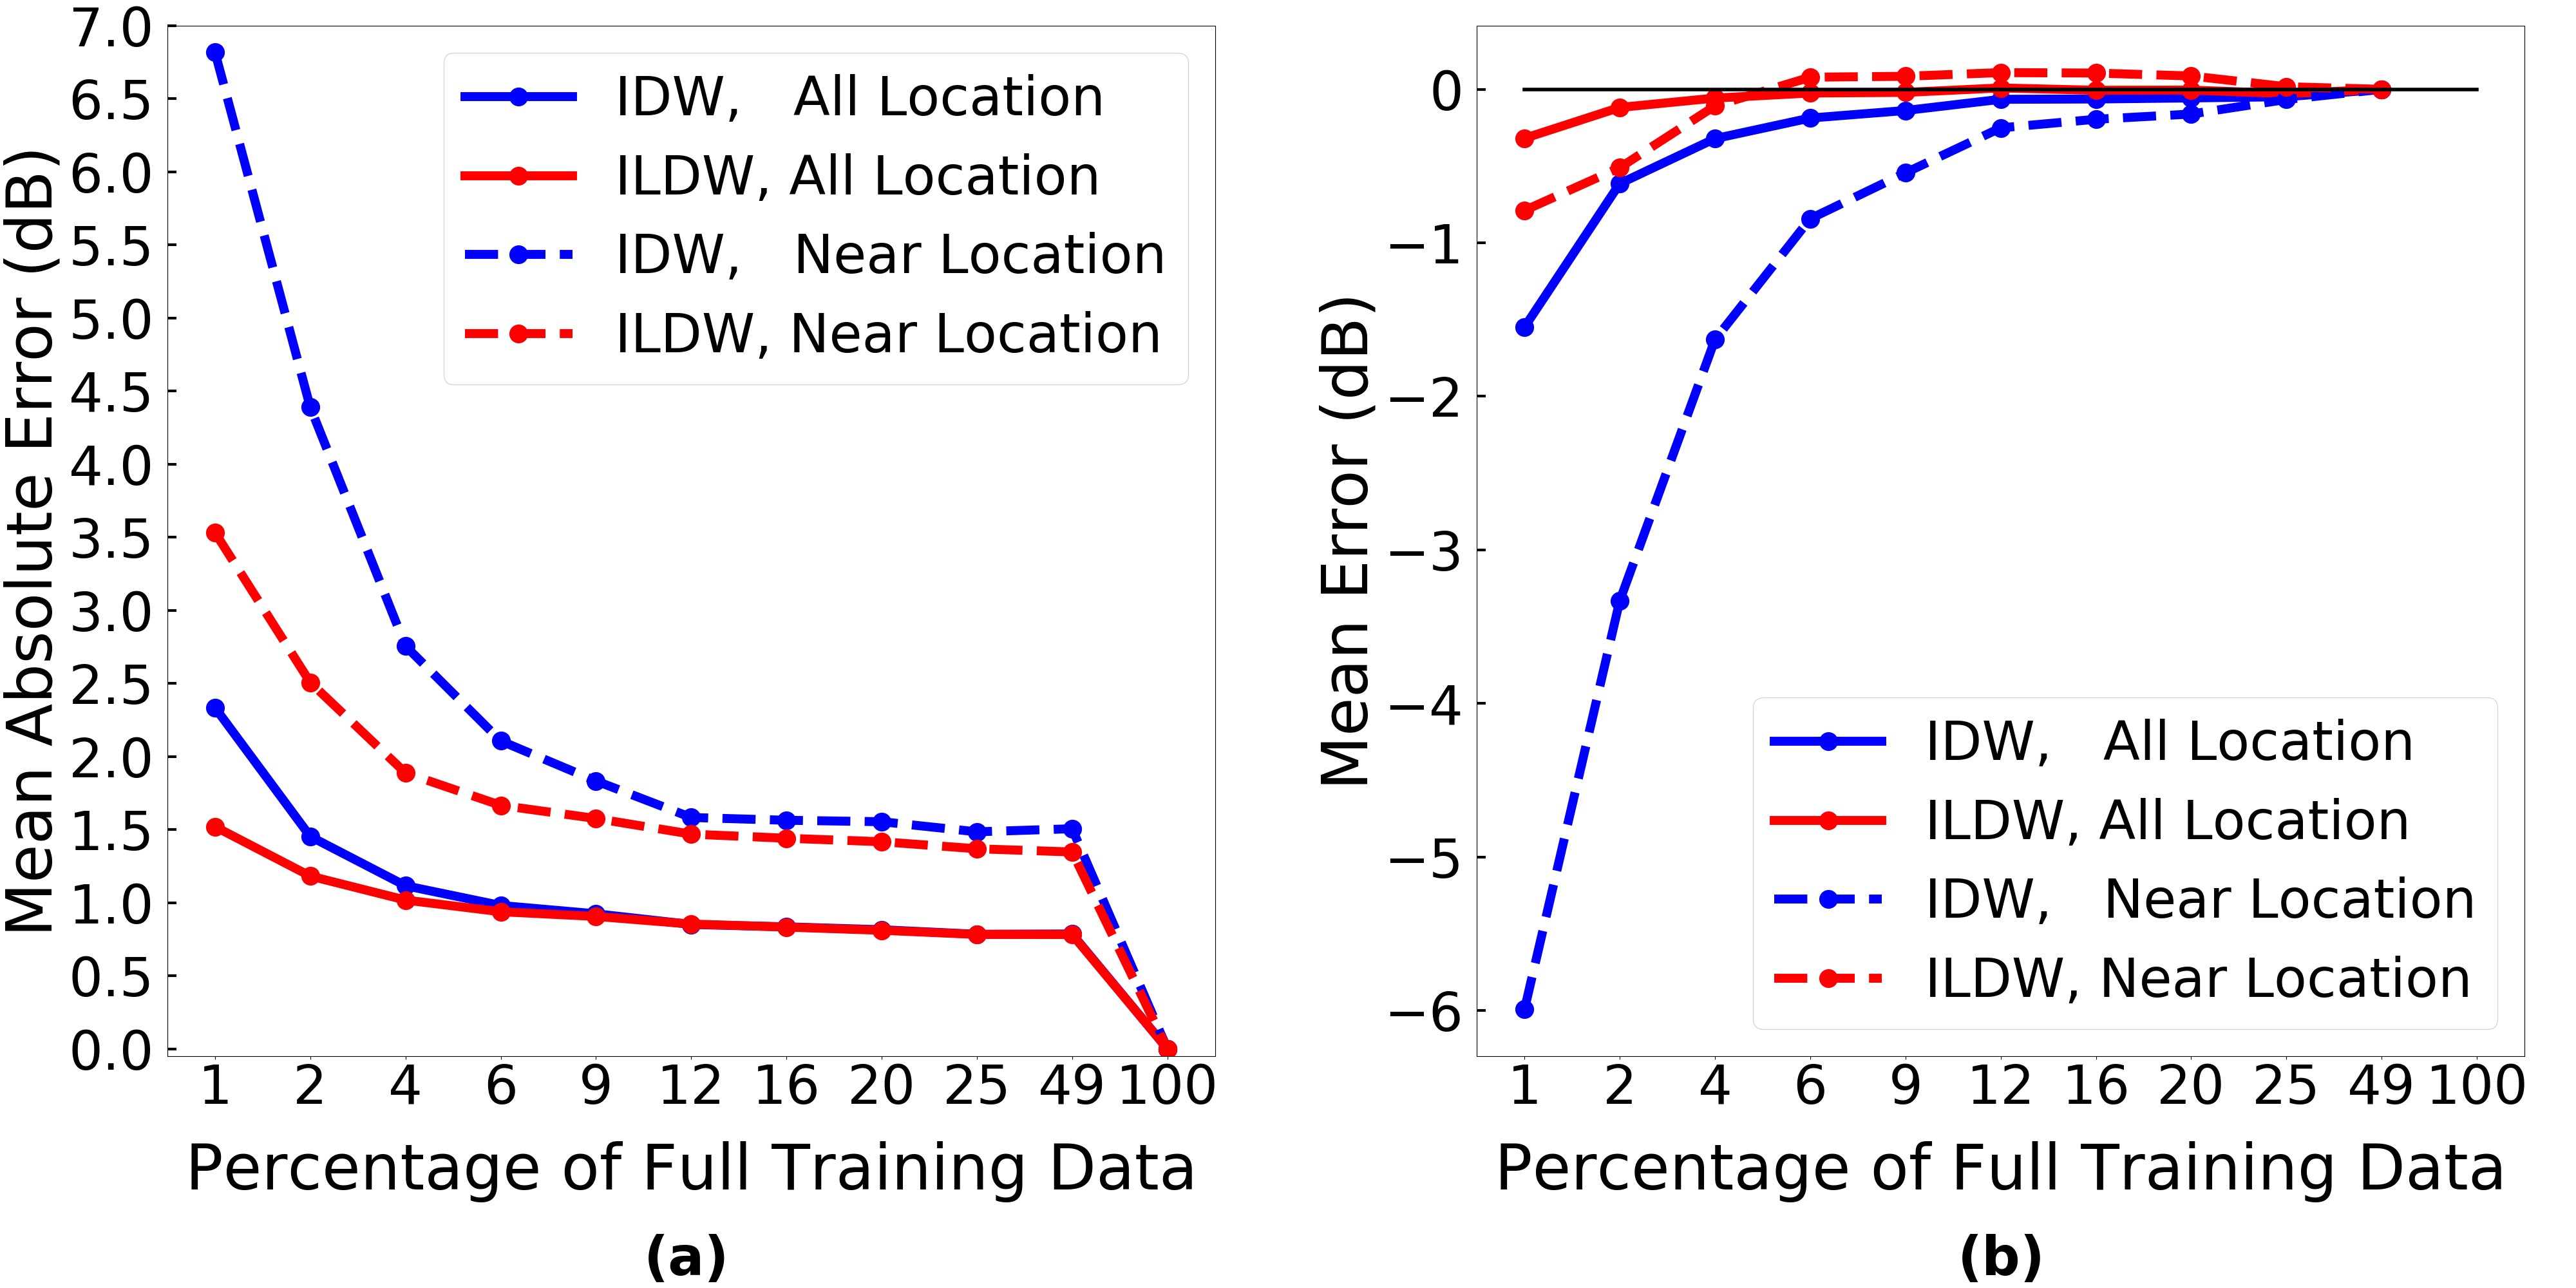
\includegraphics[width=0.8\textwidth]{chapters/ipsn/figures/inter_error.png}
	\caption{Estimation errors for interpolation schemes for varying training data}
	\label{fig:inter-error}
\end{figure}

\para{Varying Sensor Density.} We now vary the total number of sensors
in the field, and observe the impact on the performance of various
algorithms. See Figure \ref{fig:varying-num-sendensity}, where the
number of sensors is varied from 80 to 400. We see that all algorithms
perform better with increasing number of sensors as expected, with
\ouralgo performance improving significantly (in both $\lerr$ as well
as $f_r + m_r$) as number of sensors is increased from 80 to 160. More
importantly, except for very low number of sensors (i.e., 80),
\ouralgo handily outperforms the other two algorithms.


\para{Varying Training Cost.}  Finally, we now investigate how the
training cost (i.e., number of PDs constructed from raw observations)
affects the performance of our \ouralgo algorithm. Note that the other
algorithms do not depend on the training data, hence not shown.
%%%%%%%%%%
We first evaluate the interpolation error of our \ildw scheme for
varying training cost (number of known PDs) by comparing with the
traditional IDW scheme on which it is based. See
Figure~\ref{fig:inter-error}, which plots the mean absolute error
(MAE) as well as mean error (ME). As the interpolation error is
substantially higher for points that are closer to the transmitter, we
plot MAE and ME as averaged over all interpolated points as well as
over just the points close (less than 800m away) to the transmitter. Note
that the PDs at sensor locations closer to the transmitter would have
a stronger bearing on the localization accuracy, and thus, the MAE and
ME values for points closer to the transmitter are of more
significance.
%%%%%
We observe here that as expected both MAE and (absolute value of) ME
decrease with increase in the training cost for both \idw and \ildw,
but MAE and ME of \ildw is significantly lower than that of \idw
especially for low percentages of training cost and when the points
are close to the transmitter.
%\rd{HG: I want to remove the following
 % sentence.}  \ble{This shows that weighting the neighbors in the
  %logarithm scale towards the transmitter mitigates the negative
  %trend.}

We now plot the performance of \ouralgo for varying training data; see
Figure~\ref{fig:varying-training-data}. As expected, the performance
metrics show general improvement with increase in amount of
training. More importantly, we note that with 5-10\% of training,
\ouralgo achieves performance comparable to that with 100\% training,
suggesting that our interpolation scheme is largely effective as long
as 5-10\% of PDs are constructed from raw observations. 
\eat{TODO \red{Put Fig 7+8,
  9+10 in the same ROWs as Fig 7(a)-(b) and 8(a)-(b). will look better.}}



\begin{figure}[ht]
	\centering
	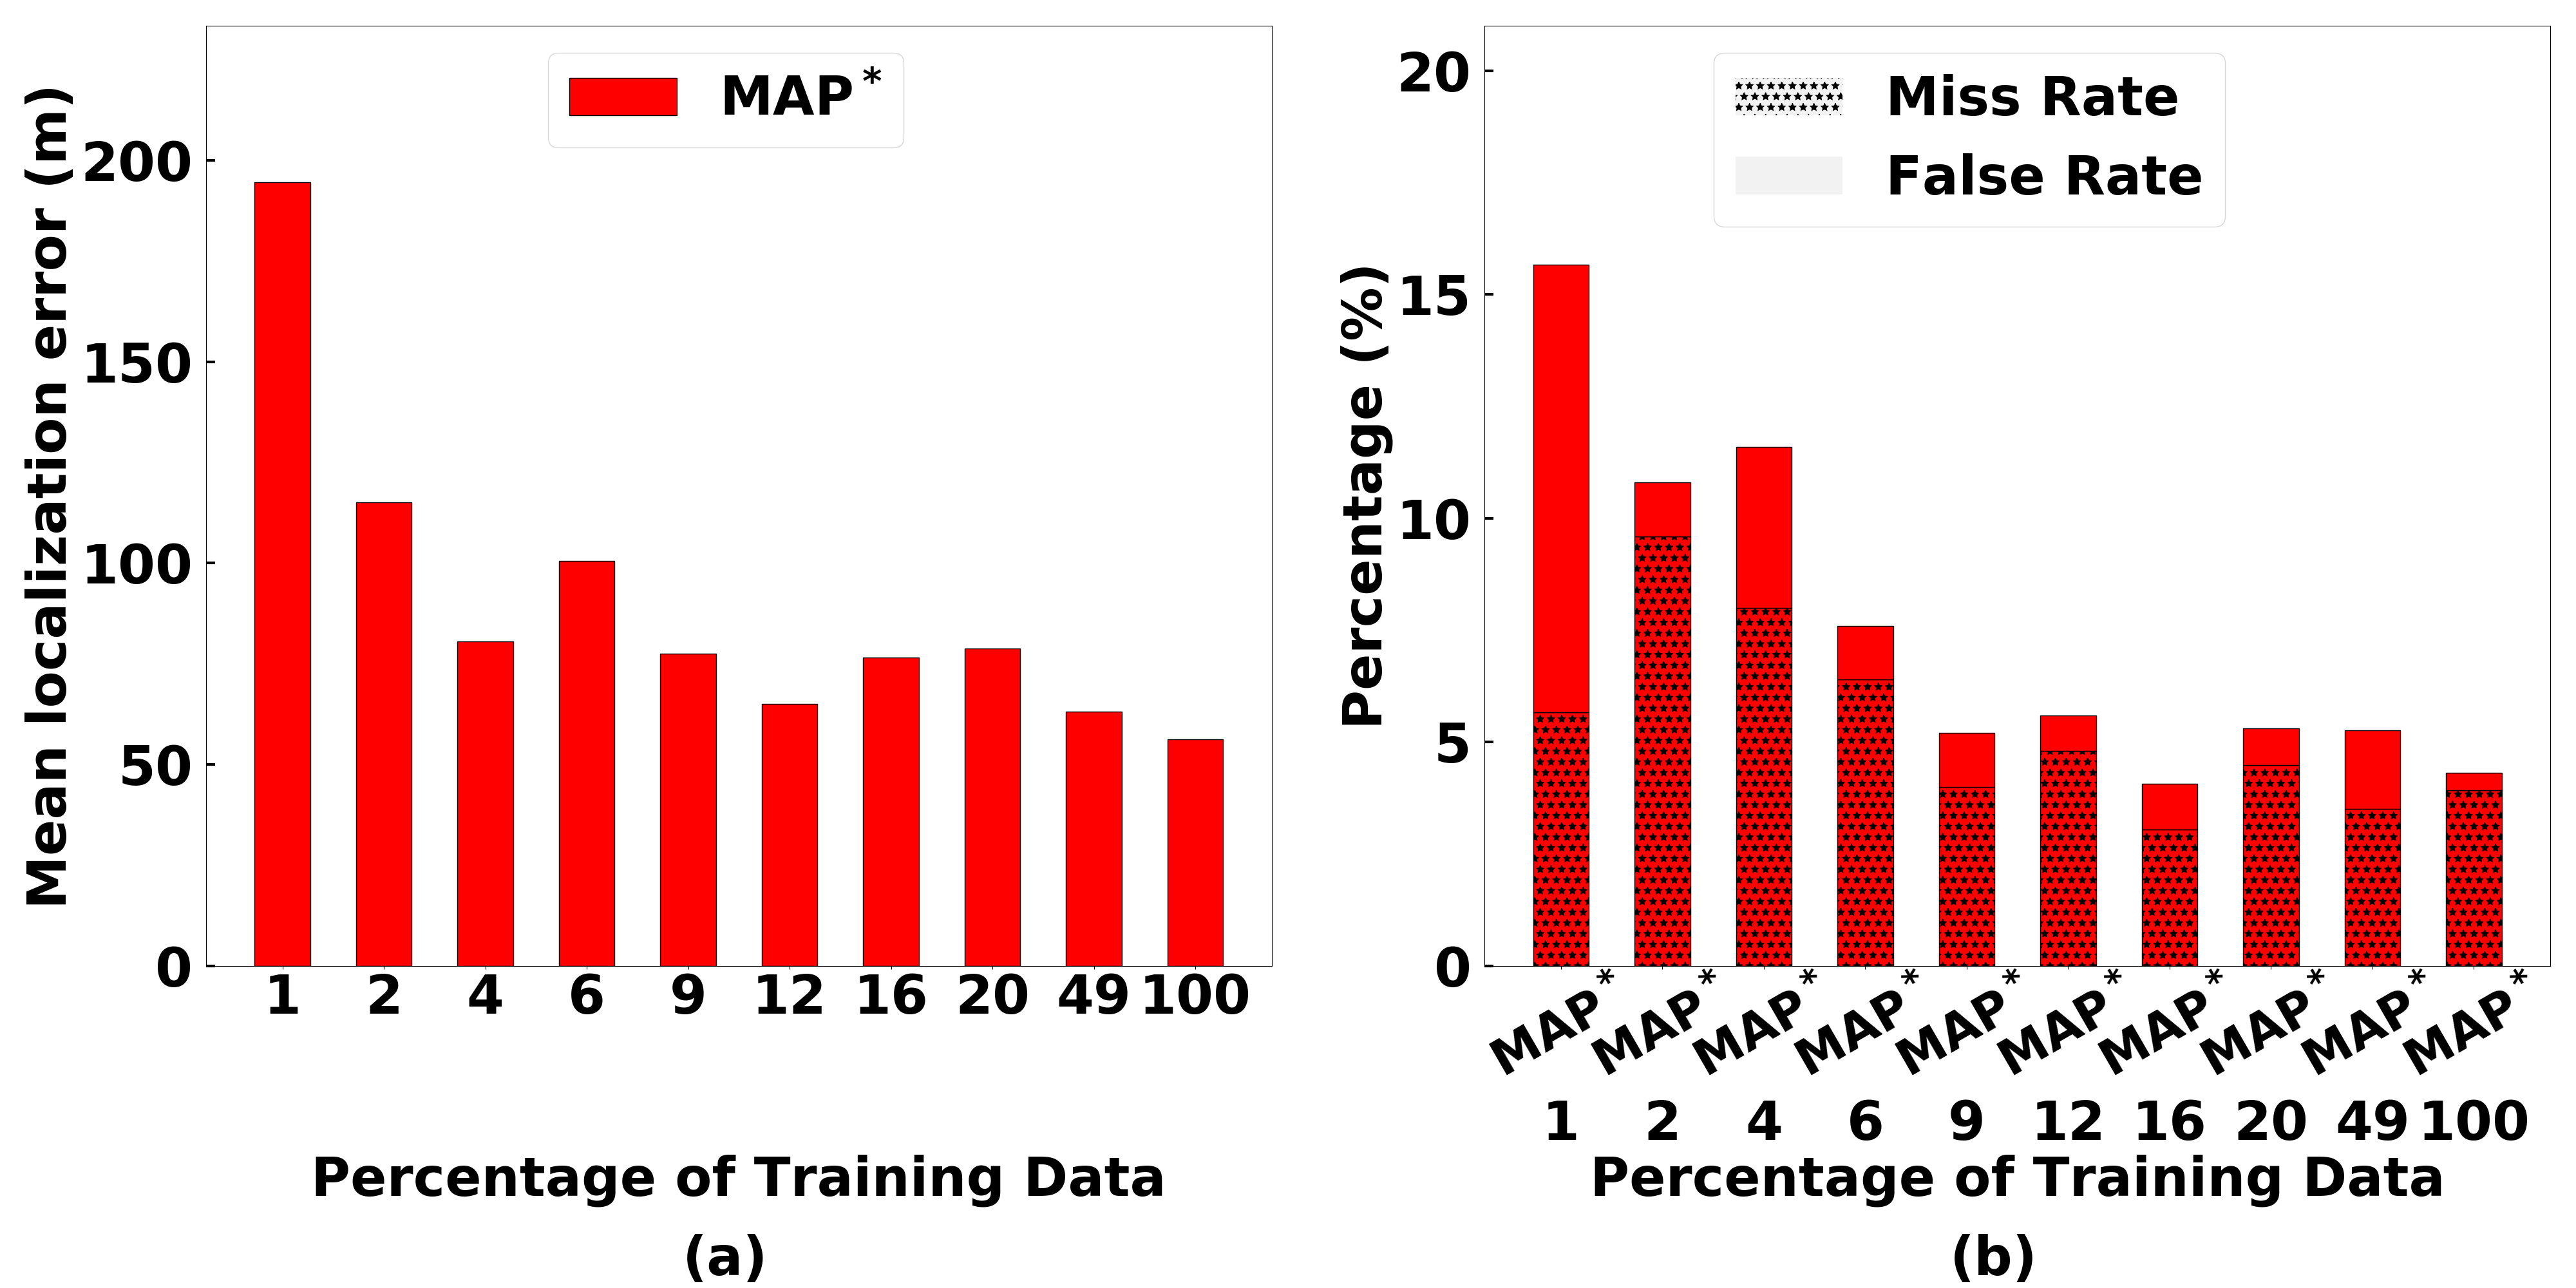
\includegraphics[width=0.8\textwidth]{chapters/ipsn/figures/splat-vary-training.png}
	\caption{Localization performance of \ouralgo in a large scale area, for varying training data}
	\label{fig:varying-training-data}
\end{figure}

\para{In Presence of Authorized Users (\ouralgoss).}  We now evaluate
the performance of our \ouralgoss approach which is tailored to work
in the presence of authorized users. To evaluate \ouralgoss, we place
5 authorized users in the area---with 2 primary and 3 secondary users.
The primary users are placed at fixed locations, while the secondaries
are put at random locations. We assign each authorized user a random
power in the range of 30 to 32dBm, while, as before, a random power
between 28 and 32dBm to the intruders. To ensure that these 5
authorized users do not ``interfere'' with each other, we ensure that
the distance between any two of these authorized users is at least
1000m.
%%%%%%%%%
We compare \ouralgoss with the simpler approach called \ouralgos that
uses \ouralgo to localize all transmitters (authorized as well as
intruders) and then removes the predicted transmitters that are
closest to the authorized users.
%%%
See Figure \ref{fig:shared-spectrum}, which shows that \ouralgoss easily
outperforms \ouralgos for varying number of intruders. 

\begin{figure}[ht]
	\centering
	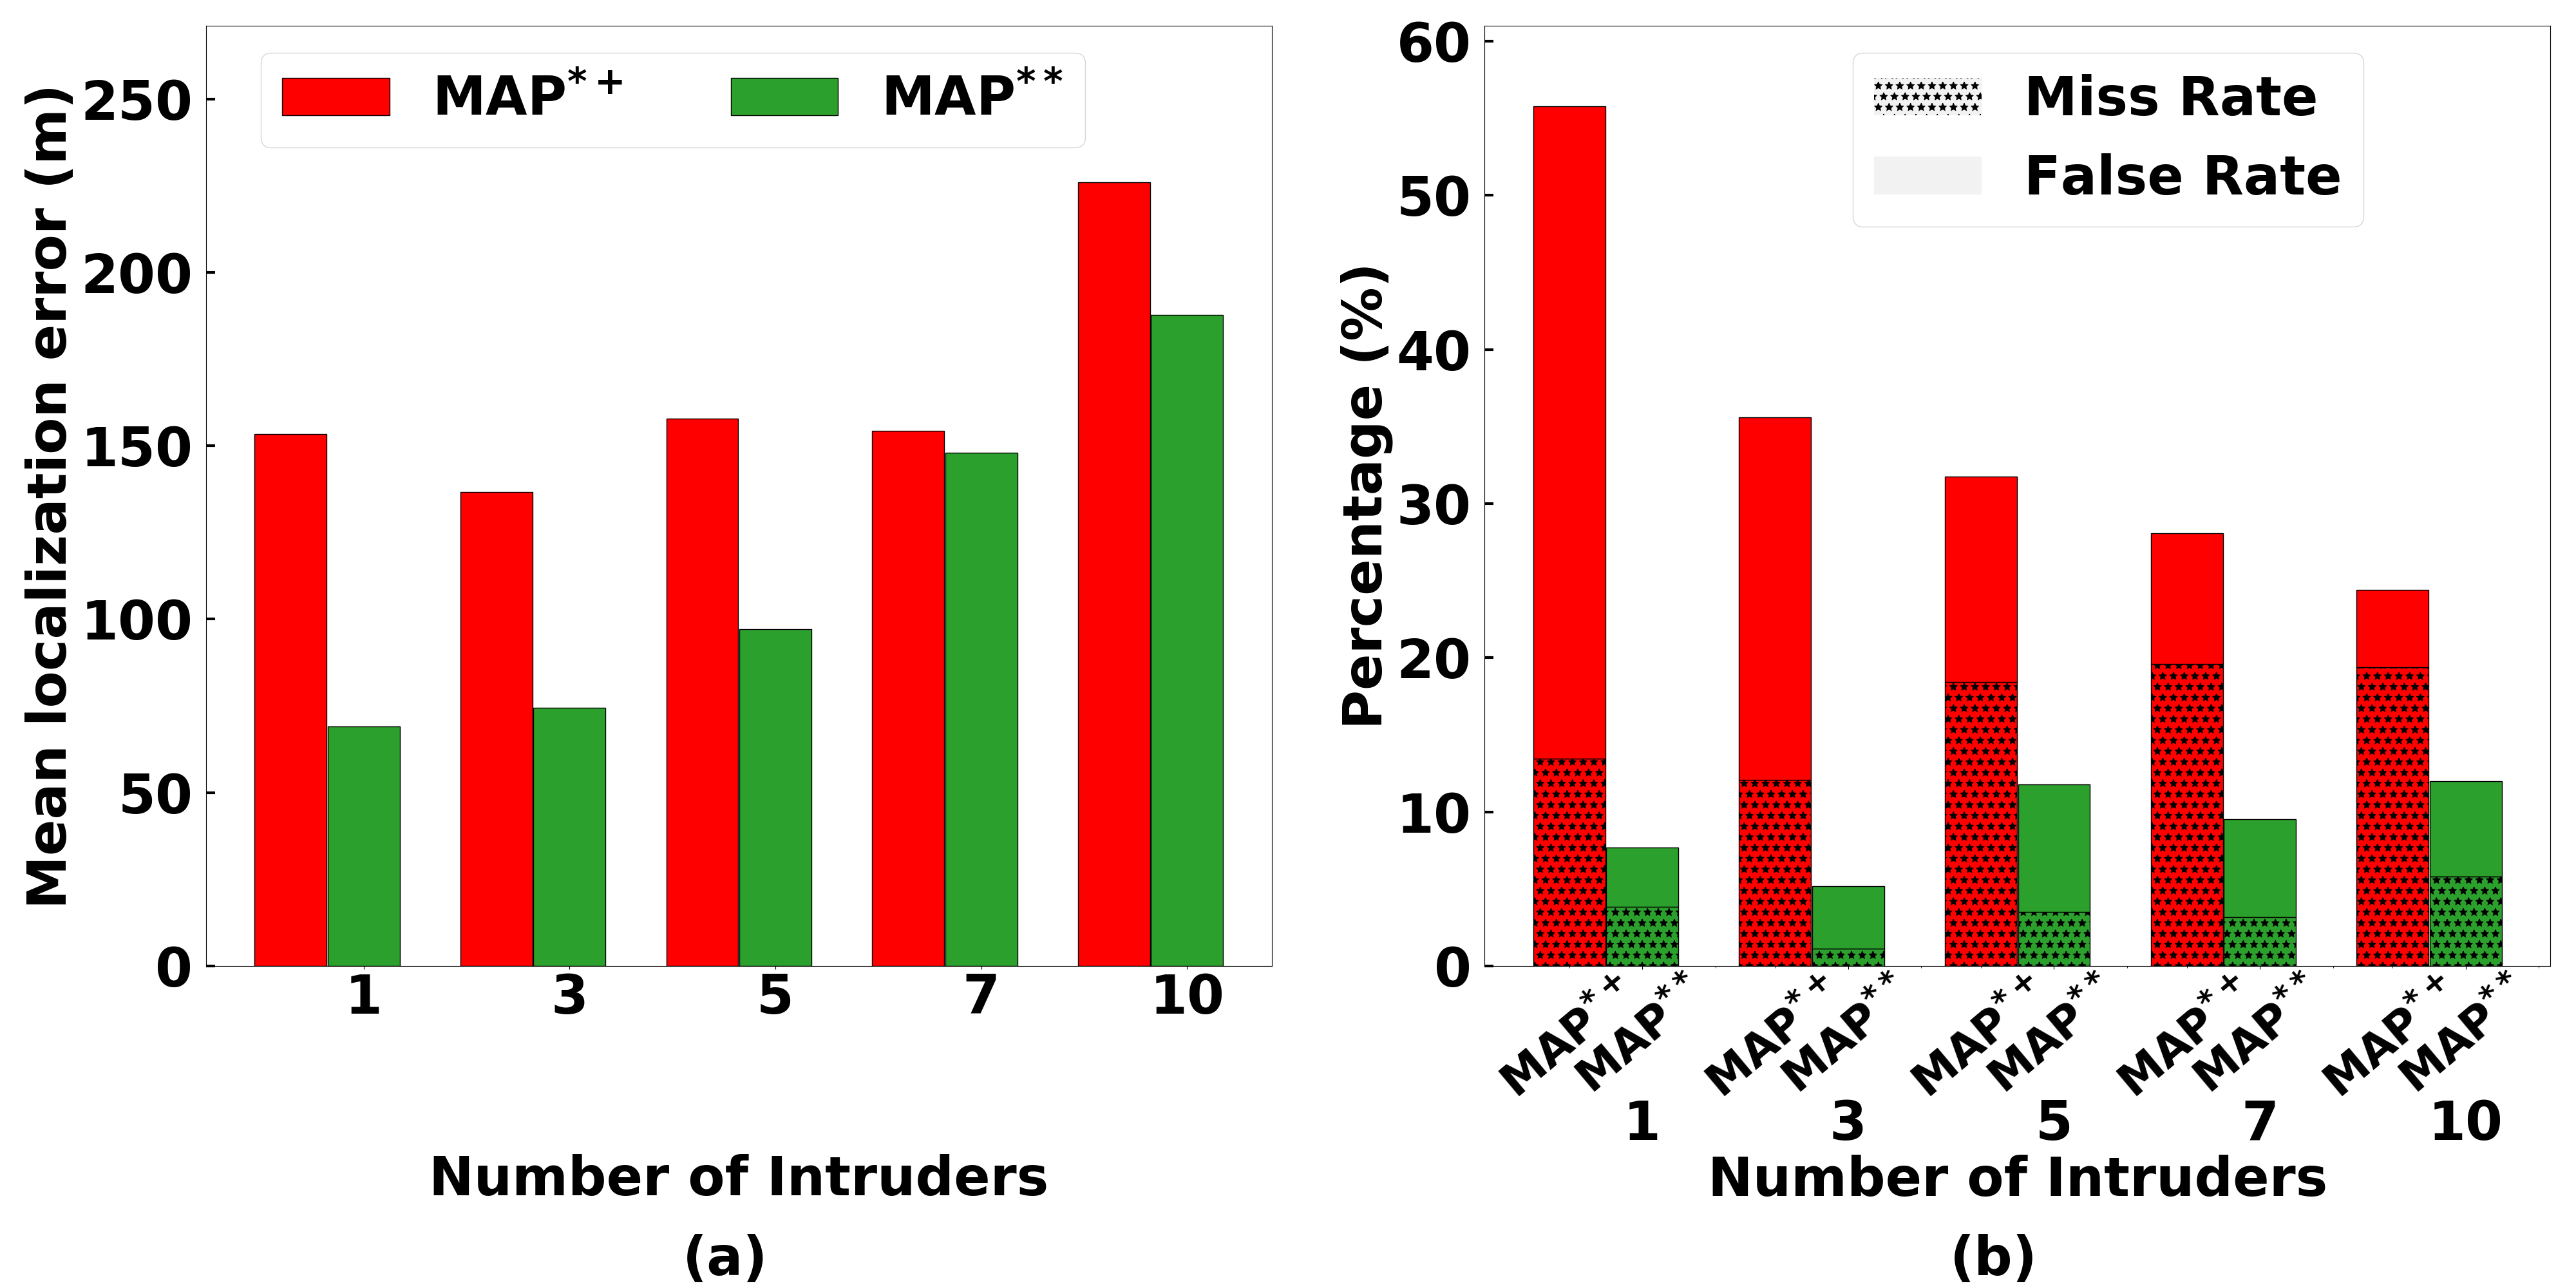
\includegraphics[width=0.8\textwidth]{chapters/ipsn/figures/splat-vary-numauthorized.png}
	\caption{Localization performance of \ouralgos and \ouralgoss in large-scale simulations with authorized users present, for varying number of intruders}
	\label{fig:shared-spectrum}
\end{figure}
